\label{sec:reveal}
\Tool currently tackles six performance anti-patterns.
While these patterns have been observed in previous work
\cite{yan:cikm17, junwen:icse2018, chen2016finding}
from real-world %severe performance problems in database-backed web
Rails applications, they have
not been systematically detected and fixed before---three anti-patterns
(RD, CS, and IA below) were automatically detected in three different frameworks; and we are unaware of prior work that performs automatic patching.

%\shan{1.This section mixes what is previous work and what is this work, which is not good: the description of each pattern should be previous work, and we should be clear about the source of each pattern; how we detect and how we fix them should be what is new about this work; 2. shouldn't ``how we will detect and how we fix'' belong to section 3? Or maybe you make this section into something like ``motivating examples'' and just pick two cases and describe in details what your tool can do, and defer in section 3 to explain what are behind the features; 3. I feel we should tell people the tool can be extended for other DB-related performance issues, is it? 4. the pattern description is too long and somewhat boring. The fact that they are not really the contribution of this tool makes it even more boring.}


\textbf{Loop invariant queries (LI)~\cite{junwen:icse2018}.} A query is repeatedly
issued in every iteration of a loop to load the \textit{same} database contents.  %Due to the nature of Ruby on Rails as a dynamic language, loop invariant query is not easy for compiler to detect and avoid. 
In the real-world example shown in 
Figure~\ref{fig:loopinv}a, hoisting the query out of the loop can speed up the 
application by more than 10$\times$ \cite{redmine23334}. 

%The program iterates through a {\tt values} list and excludes any {\tt value} field which the
%{\tt user} can only read but not write. In every iteration of the loop, the {\tt read\_only (user)} function
%is invoked to retrieves the same set of read-only fields of the user from database as shown in the Sql query in Figure~\ref{fig:loopinv}. Hoisting the invariant 
%function \textbf{read\_only (user)} out of the loop brings 20$\times$ speedup according to the developers \cite{redmine23334}.

% In traditional compiler, reaching definition is used to detect loop invariant statements.  In compiler theory, a given instruction's reaching definition is an earlier instruction whose target variable can be assigned to the given one without an intervening assignment. If  all reaching definitions one instruction are outside of the loop, the instruction can be moved out of the loop. In loop invariant query detection, we use the same concepts but limit the statement to which only will issue a query. If all reaching definition of a query  is outside the loop, then we consider this query as and loop invariant query. By hoisting the query outside the loop it previously surrounded by, we can eliminate the repeated query to be issue so as to fix this inefficiency.



\begin{figure}
\centering
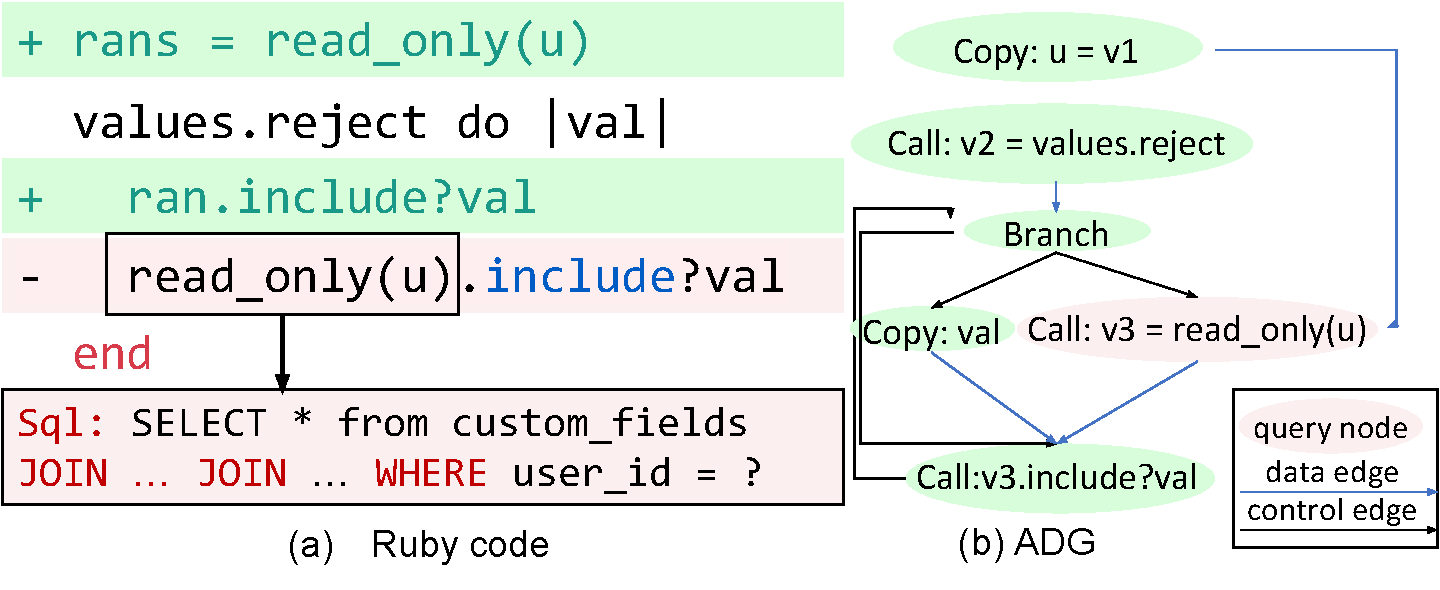
\includegraphics[width=0.8\columnwidth]{figs/redCom.pdf}

  \caption{Loop invariant query from Redmine \textmd{(the code checks which {\tt val} in {\tt values} 
  list belongs to user {\tt u}'s read-only fields})
  %\shan{the patch seems wrong}
  }
\label{fig:loopinv}
\end{figure}



\textbf{Dead store queries (DS)~\cite{junwen:icse2018}.} SQL queries are repeatedly issued to assign the same
memory object with different database contents, without any use of the memory object in between, making all but the last query unnecessary.

\textbf{Unused data-retrieval queries (RD)~\cite{chen2016finding, junwen:icse2018}.} 
Data is retrieved from the database but never 
used in the program, making the corresponding data transfer and query execution unnecessary. 

\textbf{Common sub-expression queries (CS) \cite{yan:cikm17}.} Queries with common sub-expressions are issued, causing 
unnecessary re-computation.

\textbf{API misuses (IA) \cite{junwen:icse2018}.} Different ORM APIs retrieve the same contents from the database, but they differ drastically in terms of performance.
%Our previous work \cite{junwen:icse2018}
%identified 9 such simple ORM-API misuses that do not affect functionality but hurt performance greatly. 
For example, the two Rails code snippets in Figure~\ref{fig:spreeAny} both check if a {\tt user} owns
any blog posts. However, they use different APIs, {\tt count} versus {\tt exist}, that are translated to different
SQL queries by Rails: {\tt select count} vs. {\tt select limit 1}.
The former query scans all records in the {\tt blogs} table with specified {\tt user\_id}, counts the number of records, and checks (in the Ruby application) if the count is greater than 0.
%\shan{all records or all records with specified id?} \junwen{with specified user\_id}
The latter query
returns immediately when it finds one record with the specific {\tt user\_id}, 
which can reduce query execution time by 1.7$\times$ comparing to the former.
%The latter can easily improve the resulting application performance by %1.7$\times$~\cite{junwen:icse2018}. 
%about half a second latency difference in real-world social network applications 

\begin{figure}
\centering
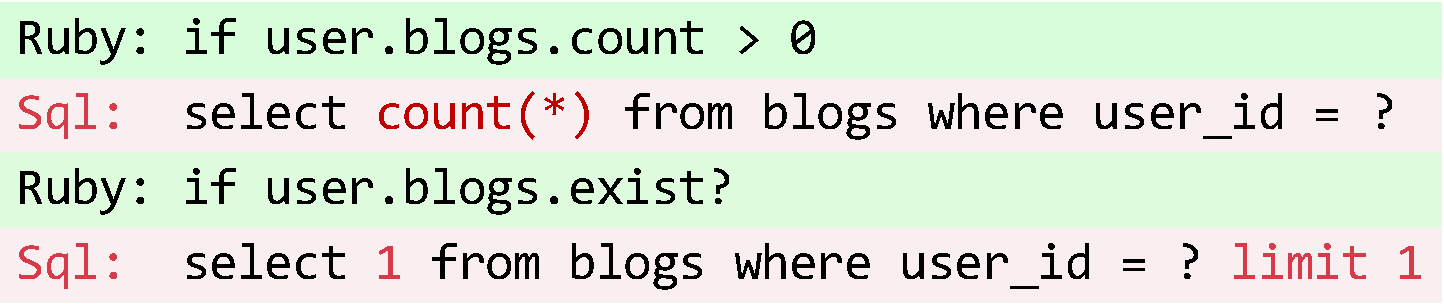
\includegraphics[width=0.6\columnwidth]{figs/api.pdf}
  
\caption{API misuse from Onebody \textmd{(the upper code is less efficient than the lower code)} %\shan{Why {\tt user\_id =1}}
}
 
\label{fig:spreeAny}
\vspace{-0.2in}
\end{figure}

\textbf{Inefficient data rendering (IR) \cite{junwen:icse2018}.} While rendering a list of objects, helper
functions are often used to render a partial view for one object at a time, with much redundant
computation repeated for every object. For example, the HTML in 
Figure \ref{fig:rendering}b is generated line by line by repeated invocations of {\tt link\_to}
with much redundancy across lines. Such inefficiency is particularly severe when there are 
many objects to render. Consequently, it could become a scalability bottleneck when
the objects need to be first retrieved from database. 
%\alvin{why this only happens after  objects are returned by db}

We find these six anti-patterns to be prevalent even in well-developed applications as 
developers are often unaware of what database
queries are issued due to the ORM abstraction. Such queries also cannot be
optimized by traditional Ruby compilers as they treat ORM APIs as
black boxes (nor database engines as they can only observe the queries issued by the application). We next explain how \Tool can detect such patterns.


%Figure~\ref{fig:sub} shows an example of statements which will issue queries that share common subexpressions. The common subexpression among two statements is \textit{projects.visible.order('id ASC')}. By caching it firstly, a better performance can be achieved. In order to detect this inefficiency, we should check whether the same query function is used in two different query function chains. If so, the corresponding queries share a common subexpression. After knowing which subexpression has been shared, we can cache the shared subexpression firstly by creating a new variable and replace the later usage of the subexpression with the new variable. We will also ensure there is no name conflict to make sure the program correctness.

%\begin{figure}[H]
%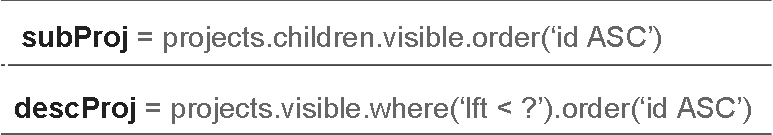
\includegraphics[width=\columnwidth]{figs/sub.pdf}
%\caption{queries share common subexpressions}
%\label{fig:sub}
%\end{figure}


\begin{comment}

\begin{table}[t]
\centering
\caption{Performance anti-patterns}
\vspace{-0.1in}
{\small
\label{tab:perfhis}
\begin{tabular}{lc@{\hspace{4pt}}c@{\hspace{4pt}}c@{\hspace{4pt}}c@{\hspace{4pt}}c@{\hspace{4pt}}c@{\hspace{4pt}}c@{\hspace{4pt}}c@{\hspace{4pt}}c@{\hspace{4pt}}c@{\hspace{4pt}}c@{\hspace{4pt}}c@{\hspace{4pt}}}
\toprule
   &\multicolumn{6}{c}{Auto-Detection} & \multicolumn{6}{c}{Auto-Fixing}\\
   \cmidrule(lr){2-7}
   \cmidrule(lr){8-13}
   & LI & DS & RD & CS & IA & IR & LI & DS & RD & CS & IA & IR    \\
\midrule
FRDA \cite{chen2016finding}& & & \cmark &&&& & & &&&&\\ 
\cite{yan:cikm17}     & & &  &\cmark&&& & & &&&&\\
\cite{junwen:icse2018}& & &  &&\cmark&& & & &&&&\\
\small{\Tool}  &\cmark&\cmark&\cmark&\cmark&\cmark&\cmark&\cmark&\cmark&\cmark&\cmark&\cmark&\cmark\\
%Loop Invariants   &  API checker\cite{junwen:icse2018} & PowerStation & PowerStation   \\
%Dead Stores   &  API checker\cite{junwen:icse2018} &PowerStation & PowerStation   \\
%Unused Data  &  FRDA\cite{chen2016finding} & FRDA\cite{chen2016finding}  & PowerStation   \\
%Common Sub-expr & AFG\cite{yan:cikm17} & AFG \cite{yan:cikm17} & N/A  \\
%API Misuses   & API checker\cite{junwen:icse2018} & API checker\cite{junwen:icse2018}  & PowerStation  \\
%Inefficient Render  &  API checker\cite{junwen:icse2018} & PowerStation  & PowerStation   \\
\bottomrule
\end{tabular}
}
\vspace{-0.1in}
\end{table}
\end{comment}